% Options for packages loaded elsewhere
\PassOptionsToPackage{unicode}{hyperref}
\PassOptionsToPackage{hyphens}{url}
\PassOptionsToPackage{dvipsnames,svgnames,x11names}{xcolor}
%
\documentclass[
]{agujournal2019}

\usepackage{amsmath,amssymb}
\usepackage{iftex}
\ifPDFTeX
  \usepackage[T1]{fontenc}
  \usepackage[utf8]{inputenc}
  \usepackage{textcomp} % provide euro and other symbols
\else % if luatex or xetex
  \usepackage{unicode-math}
  \defaultfontfeatures{Scale=MatchLowercase}
  \defaultfontfeatures[\rmfamily]{Ligatures=TeX,Scale=1}
\fi
\usepackage{lmodern}
\ifPDFTeX\else  
    % xetex/luatex font selection
\fi
% Use upquote if available, for straight quotes in verbatim environments
\IfFileExists{upquote.sty}{\usepackage{upquote}}{}
\IfFileExists{microtype.sty}{% use microtype if available
  \usepackage[]{microtype}
  \UseMicrotypeSet[protrusion]{basicmath} % disable protrusion for tt fonts
}{}
\makeatletter
\@ifundefined{KOMAClassName}{% if non-KOMA class
  \IfFileExists{parskip.sty}{%
    \usepackage{parskip}
  }{% else
    \setlength{\parindent}{0pt}
    \setlength{\parskip}{6pt plus 2pt minus 1pt}}
}{% if KOMA class
  \KOMAoptions{parskip=half}}
\makeatother
\usepackage{xcolor}
\setlength{\emergencystretch}{3em} % prevent overfull lines
\setcounter{secnumdepth}{5}
% Make \paragraph and \subparagraph free-standing
\makeatletter
\ifx\paragraph\undefined\else
  \let\oldparagraph\paragraph
  \renewcommand{\paragraph}{
    \@ifstar
      \xxxParagraphStar
      \xxxParagraphNoStar
  }
  \newcommand{\xxxParagraphStar}[1]{\oldparagraph*{#1}\mbox{}}
  \newcommand{\xxxParagraphNoStar}[1]{\oldparagraph{#1}\mbox{}}
\fi
\ifx\subparagraph\undefined\else
  \let\oldsubparagraph\subparagraph
  \renewcommand{\subparagraph}{
    \@ifstar
      \xxxSubParagraphStar
      \xxxSubParagraphNoStar
  }
  \newcommand{\xxxSubParagraphStar}[1]{\oldsubparagraph*{#1}\mbox{}}
  \newcommand{\xxxSubParagraphNoStar}[1]{\oldsubparagraph{#1}\mbox{}}
\fi
\makeatother


\providecommand{\tightlist}{%
  \setlength{\itemsep}{0pt}\setlength{\parskip}{0pt}}\usepackage{longtable,booktabs,array}
\usepackage{calc} % for calculating minipage widths
% Correct order of tables after \paragraph or \subparagraph
\usepackage{etoolbox}
\makeatletter
\patchcmd\longtable{\par}{\if@noskipsec\mbox{}\fi\par}{}{}
\makeatother
% Allow footnotes in longtable head/foot
\IfFileExists{footnotehyper.sty}{\usepackage{footnotehyper}}{\usepackage{footnote}}
\makesavenoteenv{longtable}
\usepackage{graphicx}
\makeatletter
\newsavebox\pandoc@box
\newcommand*\pandocbounded[1]{% scales image to fit in text height/width
  \sbox\pandoc@box{#1}%
  \Gscale@div\@tempa{\textheight}{\dimexpr\ht\pandoc@box+\dp\pandoc@box\relax}%
  \Gscale@div\@tempb{\linewidth}{\wd\pandoc@box}%
  \ifdim\@tempb\p@<\@tempa\p@\let\@tempa\@tempb\fi% select the smaller of both
  \ifdim\@tempa\p@<\p@\scalebox{\@tempa}{\usebox\pandoc@box}%
  \else\usebox{\pandoc@box}%
  \fi%
}
% Set default figure placement to htbp
\def\fps@figure{htbp}
\makeatother

\usepackage{url} %this package should fix any errors with URLs in refs.
\usepackage{lineno}
\usepackage[inline]{trackchanges} %for better track changes. finalnew option will compile document with changes incorporated.
\usepackage{soul}
\linenumbers
\makeatletter
\@ifpackageloaded{caption}{}{\usepackage{caption}}
\AtBeginDocument{%
\ifdefined\contentsname
  \renewcommand*\contentsname{Table of contents}
\else
  \newcommand\contentsname{Table of contents}
\fi
\ifdefined\listfigurename
  \renewcommand*\listfigurename{List of Figures}
\else
  \newcommand\listfigurename{List of Figures}
\fi
\ifdefined\listtablename
  \renewcommand*\listtablename{List of Tables}
\else
  \newcommand\listtablename{List of Tables}
\fi
\ifdefined\figurename
  \renewcommand*\figurename{Figure}
\else
  \newcommand\figurename{Figure}
\fi
\ifdefined\tablename
  \renewcommand*\tablename{Table}
\else
  \newcommand\tablename{Table}
\fi
}
\@ifpackageloaded{float}{}{\usepackage{float}}
\floatstyle{ruled}
\@ifundefined{c@chapter}{\newfloat{codelisting}{h}{lop}}{\newfloat{codelisting}{h}{lop}[chapter]}
\floatname{codelisting}{Listing}
\newcommand*\listoflistings{\listof{codelisting}{List of Listings}}
\makeatother
\makeatletter
\makeatother
\makeatletter
\@ifpackageloaded{caption}{}{\usepackage{caption}}
\@ifpackageloaded{subcaption}{}{\usepackage{subcaption}}
\makeatother

\usepackage{bookmark}

\IfFileExists{xurl.sty}{\usepackage{xurl}}{} % add URL line breaks if available
\urlstyle{same} % disable monospaced font for URLs
\hypersetup{
  pdftitle={Arizona Aquifer Recharge Suitability Analysis},
  pdfauthor={Travis Zalesky},
  pdfkeywords={Arizona Tri University Recharge (ATUR), water
table, ground water},
  colorlinks=true,
  linkcolor={blue},
  filecolor={Maroon},
  citecolor={Blue},
  urlcolor={Blue},
  pdfcreator={LaTeX via pandoc}}



\draftfalse

\begin{document}
\title{Arizona Aquifer Recharge Suitability Analysis}

\authors{Travis Zalesky\affil{1}}
\affiliation{1}{University of Arizona, }
\correspondingauthor{Travis Zalesky}{travisz@arizona.edu}


\begin{abstract}
Aquifer recharge can be either passive or active, and is implemented in
a variety of ways. This analysis seeks to identify regions across AZ
which are boadly suitable for aquifer recharge projects as a general
template for more focuse analysis.
\end{abstract}

\section*{Plain Language Summary}
Identifying regions in AZ where surface water can be stored long-term as
ground water.




\section{Introduction}\label{introduction}

\section{Data \& Methods}\label{sec-data-methods}

\textbf{These methods and data layers are preliminary and subject to
change} \#\#\# Elevation \#\#\#\# DEM Elevation and elevation
derivatives from 30-m NASA SRTM. USGS 3-DEM (10m) product not suitable
for full study area analysis due to (1) the large area of missing data
in Mexico, and (2), the excessively high spatial resolution (massively
increasing computational requirements).

SRTM elevation sinks filled prior to calculating slope and aspect.

\textbf{Should elevation be directly used in the suitability analysis?}

\subsubsection{Slope}\label{slope}

Slope derived from hydrologically conditioned (filled) 30-m SRTM layer
using quadratic surface function and a fixed 30-m neighborhood. Slope
measured in °.

\begin{quote}
Higher slopes are less suitable because thinning is both more expensive
and more precipitation will end up as runoff.
\end{quote}

Slope classified from 1-10 using a \textbf{continuous function} in
ArcPro Suitability Mapper.

\begin{longtable}[]{@{}
  >{\centering\arraybackslash}p{(\linewidth - 2\tabcolsep) * \real{0.3750}}
  >{\centering\arraybackslash}p{(\linewidth - 2\tabcolsep) * \real{0.6250}}@{}}
\toprule\noalign{}
\begin{minipage}[b]{\linewidth}\centering
Pamameter
\end{minipage} & \begin{minipage}[b]{\linewidth}\centering
Setting
\end{minipage} \\
\midrule\noalign{}
\endhead
\bottomrule\noalign{}
\endlastfoot
Function &
\href{https://pro.arcgis.com/en/pro-app/latest/tool-reference/spatial-analyst/the-transformation-functions-available-for-rescale-by-function.htm\#ESRI_SECTION1_6C2FDA23D8094B8F99DBF3DF5E176B1D}{MSSSmall} \\
Mean multiplyer & 1 \\
Sddv multiplier & 2 \\
Lower threshold & 0 \\
Value below threshold & 0 \\
Upper threshold & 90 \\
Value above threshold & 0 \\
Invert function & FALSE \\
Save transformed dataset & TRUE \\
Output & Transformed\_SRTM\_slope \\
\end{longtable}

\begin{figure}[H]

{\centering \pandocbounded{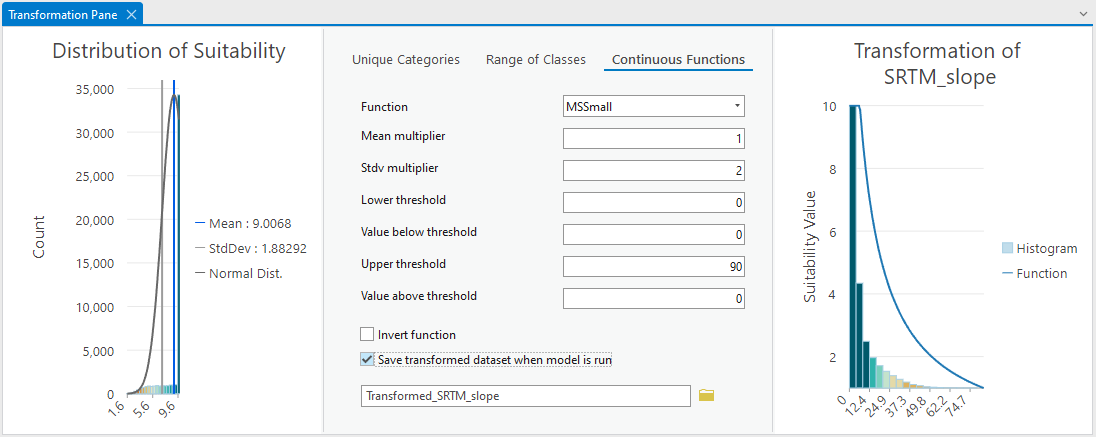
\includegraphics[keepaspectratio]{images/SuitabilityAnalysis_Transformations/Slope.png}}

}

\caption{Slope suitability mapper rescale transformation setup.}

\end{figure}%

\subsubsection{Aspect}\label{aspect}

Aspect calculated as with slope. Aspect reference point at N. Pole.

\begin{quote}
Aspect has a large impact on solar radiation.
\end{quote}

\begin{quote}
Closer to 0 or 360 is desired, low suitability scores for closeness.
\end{quote}

Aspect classified from 1-10 using a \textbf{continuous function} in
ArcPro Suitability Mapper.

\begin{longtable}[]{@{}
  >{\centering\arraybackslash}p{(\linewidth - 2\tabcolsep) * \real{0.3750}}
  >{\centering\arraybackslash}p{(\linewidth - 2\tabcolsep) * \real{0.6250}}@{}}
\toprule\noalign{}
\begin{minipage}[b]{\linewidth}\centering
Pamameter
\end{minipage} & \begin{minipage}[b]{\linewidth}\centering
Setting
\end{minipage} \\
\midrule\noalign{}
\endhead
\bottomrule\noalign{}
\endlastfoot
Function &
\href{https://pro.arcgis.com/en/pro-app/latest/tool-reference/spatial-analyst/the-transformation-functions-available-for-rescale-by-function.htm\#ESRI_SECTION1_A7FC2FC126CD4A41974C8D3F5E0F8FD6}{Near} \\
Mid Point & 180 \\
Point spread & 0.0011049638968393428 (default) \\
Lower threshold & -1 (flat) \\
Value below threshold & 0 \\
Upper threshold & 360 \\
Value above threshold & 0 \\
Invert function & TRUE \\
Save transformed dataset & TRUE \\
Output & Transformed\_SRTM\_aspect \\
\end{longtable}

\begin{figure}[H]

{\centering \pandocbounded{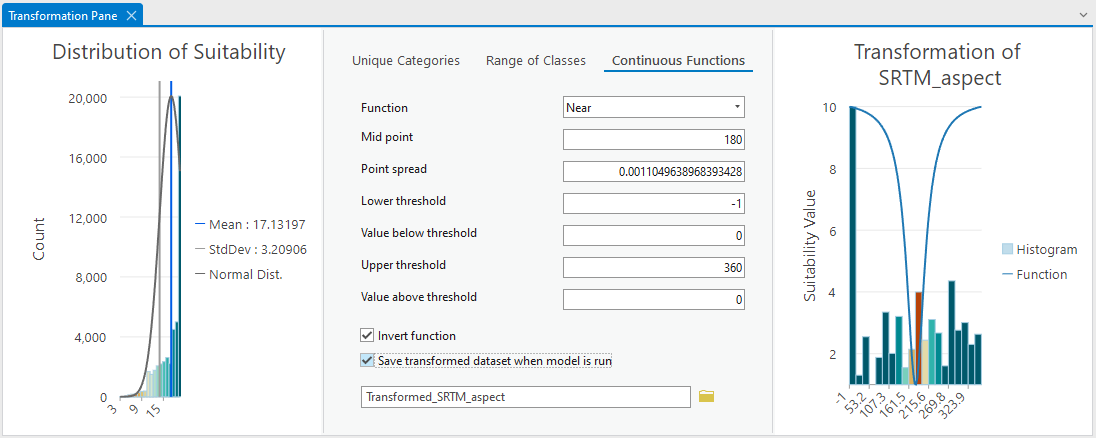
\includegraphics[keepaspectratio]{images/SuitabilityAnalysis_Transformations/Aspect.png}}

}

\caption{Aspect suitability mapper rescale transformation setup.}

\end{figure}%

\subsection{Precipitation}\label{precipitation}

PRISM normals, 800m resolution. Annual precipitation.

\begin{quote}
Mean annual precipitation must be higher than 500mm 1990 - 2020
\end{quote}

Precipitation classified from 1-10 using a \textbf{continuous function}
in ArcPro Suitability Mapper.

NOTE: The logistic growth function may also be a good choice for this
dataset. See
\href{https://pro.arcgis.com/en/pro-app/latest/tool-reference/spatial-analyst/the-transformation-functions-available-for-rescale-by-function.htm\#ESRI_SECTION1_76ED0A2D02A24C95B98B8A691603F2F4}{Logistic
Growth function}

\begin{longtable}[]{@{}
  >{\centering\arraybackslash}p{(\linewidth - 2\tabcolsep) * \real{0.3750}}
  >{\centering\arraybackslash}p{(\linewidth - 2\tabcolsep) * \real{0.6250}}@{}}
\toprule\noalign{}
\begin{minipage}[b]{\linewidth}\centering
Pamameter
\end{minipage} & \begin{minipage}[b]{\linewidth}\centering
Setting
\end{minipage} \\
\midrule\noalign{}
\endhead
\bottomrule\noalign{}
\endlastfoot
Function &
\href{https://pro.arcgis.com/en/pro-app/latest/tool-reference/spatial-analyst/the-transformation-functions-available-for-rescale-by-function.htm\#ESRI_SECTION1_B83C9047549542DE995823E6030A29F3}{MSLarge} \\
Mean multiplyer & 1.68 (aproximates 500mm at x-intercept) \\
Sddv multiplier & 1 \\
Lower threshold & 67.33789825439453 (default, minimum) \\
Value below threshold & 0 \\
Upper threshold & 1214.5689697265625 (default, maximum) \\
Value above threshold & 0 \\
Invert function & FALSE \\
Save transformed dataset & TRUE \\
Output & Transformed\_PRISM\_ppt\_30yrnormal\_800m \\
\end{longtable}

\begin{figure}[H]

{\centering \pandocbounded{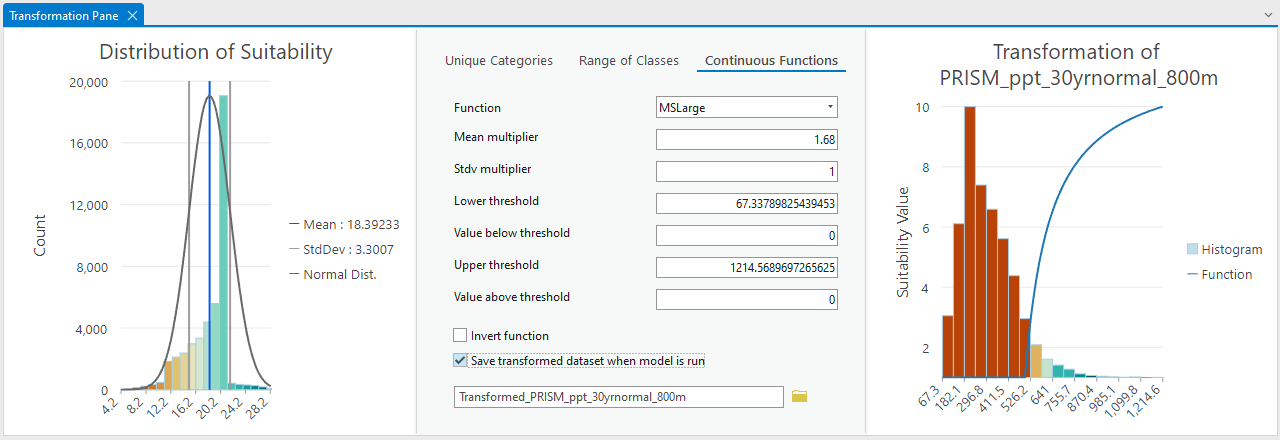
\includegraphics[keepaspectratio]{images/SuitabilityAnalysis_Transformations/Precip_PRISM.png}}

}

\caption{Aspect suitability mapper rescale transformation setup.}

\end{figure}%

\subsection{Vegetation
Characteristics}\label{vegetation-characteristics}

\subsubsection{NLCD 2021 Total Canopy
Cover}\label{nlcd-2021-total-canopy-cover}

\subsubsection{Landfire}\label{landfire}

\subsection{Soil Hydrology}\label{soil-hydrology}

AZ\_Soil\_Hydric\_Group data layer

\textbf{Classification Schema}

\begin{longtable}[]{@{}
  >{\centering\arraybackslash}p{(\linewidth - 6\tabcolsep) * \real{0.1591}}
  >{\centering\arraybackslash}p{(\linewidth - 6\tabcolsep) * \real{0.1591}}
  >{\centering\arraybackslash}p{(\linewidth - 6\tabcolsep) * \real{0.5227}}
  >{\centering\arraybackslash}p{(\linewidth - 6\tabcolsep) * \real{0.1591}}@{}}
\toprule\noalign{}
\begin{minipage}[b]{\linewidth}\centering
Class
\end{minipage} & \begin{minipage}[b]{\linewidth}\centering
Count (pixels)
\end{minipage} & \begin{minipage}[b]{\linewidth}\centering
Text
\end{minipage} & \begin{minipage}[b]{\linewidth}\centering
Value
\end{minipage} \\
\midrule\noalign{}
\endhead
\bottomrule\noalign{}
\endlastfoot
A & 62559472 & Group A soils consist of deep, well drained sands or
gravelly sands with high infiltration and low runoff rates. & 10 \\
B & 76665198 & Group B soils consist of deep well drained soils with a
moderately fine to moderately coarse texture and a moderate rate of
infiltration and runoff. & 10 \\
C & 88491710 & Group C consists of soils with a layer that impedes the
downward movement of water or fine textured soils and a slow rate of
infiltration. & 8 \\
D & 155095790 & Group D consists of soils with a very slow infiltration
rate and high runoff potential. This group is composed of clays that
have a high shrink-swell potential, soils with a high water table, soils
that have a clay pan or clay layer at or near the surface, and soils
that are shallow over nearly impervious material. & 3 \\
A/D & 43192 & Group A/D soils naturally have a very slow infiltration
rate due to a high water table but will have high infiltration and low
runoff rates if drained. & ?? \\
B/D & 18456 & Group B/D soils naturally have a very slow infiltration
rate due to a high water table but will have a moderate rate of
infiltration and runoff if drained. & ?? \\
C/D & 217771 & Group C/D soils naturally have a very slow infiltration
rate due to a high water table but will have a slow rate of infiltration
if drained. & ?? \\
\end{longtable}

\section{Conclusion}\label{sec-conclusions}

\section*{References}\label{references}
\addcontentsline{toc}{section}{References}




\end{document}
